%\documentclass{beamer}
\documentclass[handout]{beamer}

\usepackage{pgfpages} 

%\setbeameroption{show only notes}

\usetheme{default}

\mode<presentation> {
%  \usetheme{Warsaw}
  \usetheme{Frankfurt}
%  \usetheme{Boadilla}
%  \usetheme{Marburg}
}

\mode<handout>{\setbeamercolor{background canvas}{bg=black!5} %
    \pgfpagesuselayout{4 on 1}[letterpaper,border shrink=4mm,landscape] %
    \setbeameroption{show notes}}

\title[CAC High Performance Math] {High Performance Math}
\author{Brock Palen\\ \texttt{brockp@umich.edu}}
\date{TBD}

\begin{document}
  \setbeamercovered{transparent}  
  \begin{frame}
    \titlepage
  \end{frame}

%table of contents
  \begin{frame}{Outline}
    \tableofcontents
  \end{frame}
 
\begin{frame}{References}
 \begin{block}{References}
  \begin{itemize}
   \item U.C. Berkeley CS267 Jim Demmel \\
     \url{http://www.cs.berkeley.edu/~demmel/cs267/}
   \item Numerical Algorithms Group     \\
     \url{http://www.nag.com/lapack-ex/}
   \item Basic Linear Algebra Subprograms \\
     \url{http://www.netlib.org/blas/}
   \item Linear ALgebra Package         \\
     \url{http://www.netlib.org/lapack/}
  \end{itemize}
 \end{block}
 \note{
   All Traning docs are available at \url{www.umich.edu/~brockp} \\
 } %end note
\end{frame} 



\section{Concepts}
\subsection{Terms}
\begin{frame}{Terms}
 \begin{block}{Terms}
  \begin{itemize}
   \item<1-> Bandwidth - Speed in GB/s of memory to CPU
   \item<2-> Floating Point Number - Floats and Doubles (1.2 5.002)
   \item<2-> Fixed Point Number - Ints (1 50 1,000)
   \item<3-> Floating Point Operation (Flop) - A mathematic operation on a floating point number
   \item<4-> Memory Refernce - A call to memory for data
   \item<5->  $q=f/m$ - Ratio of Flops to Refernces
   \item<6-> Cache - Fast memory local to the cpu
  \end{itemize}
 \end{block}
 \note{
  Most HPC applications require floating point calculations thus focus is on FLOPS and not fixed point performance. \\
  Data in cache is assumed to be latency free. It is also assumed to have enough bandwidth to feed the CPU.
 } %end note
\end{frame}
 \subsection {Memory vs CPU}
 \begin{frame}{CPU Speed}
  \begin{block}{CPU Perfromance}
   \begin{itemize}
    \item <1->Moore's Law
    \item <2->Focus and Rightly So
    \item <3->Multi-Core
    \item <4->Single Instruction Multiple Data (Vector)
   \end{itemize}
  \end{block}
  \note{
  \url{http://en.wikipedia.org/wiki/Moore's\_law} \\
  \url{http://en.wikipedia.org/wiki/SIMD}         \\
  \url{http://en.wikipedia.org/wiki/Vector\_processor} \\
  SIMD (SSE, 3DNow, AltiVec) is related to the vector CPU's systems like the NEC SX-9.  Vectors are for working on lists of numbers at the same time. It can be thought as a type of paralellism.  Most HPC Math Libraries make use of the SIMD unit on modern CPU's.  For example on the AMD Barcilona perfromance doubled in the SIMD (sse 128) unit. \\
  SIMD is very related to GP-GPU processing and CPU's like the IBM Cell. \\
 
  Cell CPU (PS3 and Road Runner)\\ 
  \url{http://en.wikipedia.org/wiki/Cell\_microprocessor} \\
  Computed Unified Device Arch. GP-GPU for Nvidia Cards
  \url{http://en.wikipedia.org/wiki/CUDA}
  } %end note
 \end{frame}

 \begin{frame}{Memory Speed}
  \begin{block}{Memory Performance}
   \begin{itemize}
    \item <1-> Memory Size
    \item <2-> Memory Speed (GB/s) trails CPU Flops
    \item <3-> Memory Latency is Worse than You think
   \end{itemize}
  \end{block}
 \end{frame}
 \note{
  Memory speeds matter more than latency. Modern CPUs like the AMD Opteron have the memory controler right in the cpu. This lowers memory latency.  It also adds total bandwidth (speed in GB/s) for an entire system in an SMP system. In such systems memory needs to be balanced across CPU Stockets.  
 } %end note
 \begin{frame}{Human vs. Computer}
   \[
    \alpha A=c
   \]
  \begin{block}{Sacle A Vector}
   \begin{itemize}
    \item<2-> 2n Flops
    \item<3-> 3n Refernces
    \item<4-> q=2/3
    \item<5-> \alert{Memory must be faster than the CPU}
   \end{itemize}
  \end{block}
 \end{frame}
 \note{
   While using sequences of simple operations like $AB=c$ and $ \alpha B=c$ are simple for a human to have organized it is a very slow type of operation for a computer. Computers need oprotunites for data reuse. \\
   BLAS 1 Functions: \\
   $AB=c$ is xDOT()  \\
   $\alpha B=c$ is xSCAL() \\
 These are the slowest of the BLAS operations.  Their ratio $ q=f/m $ is 2/3
 } %end note

\begin{frame}{Computers are Faster}
  \[ M[ \ddots ] A[\vdots] = B[\vdots]\]
 \begin{block}{xGEMV() Matrix Vector Multiplication}
  \begin{itemize}
   \item $ 2n^2 $ Flops
   \item $n^2+n $ Refernces
   \item $q=2$
  \end{itemize}
 \end{block}
 \note{
   These are the Blas 2 operations. They require that memory be half the speed of the CPU. We will see latter how in real world examples that because Blas 2 (and Blas 1) that there is not enough data reuse (none really) to allow the cache to keep the CPU fed.
 } % end note
\end{frame}

\begin{frame}{Computers are Faster Ctd.}
 \[ M[ \ddots ] N[ \ddots ] = C[ \ddots ] \]
 \begin{block}{xGEMM() Matrix Matrix Multiplication}
  \begin{itemize}
   \item $ 2n^3 \rightarrow n^3 $ Flops
   \item $ 4n^2 $ Refernces
   \item $ q=n/2 $
  \end{itemize}
 \end{block}
\end{frame}
 \note{
  Blas 3.  These calls are the basis of the LAPACK calls. Notice how as the size of M scales the ratio of flops (when coded right) increases to memory references.  The reason for this is clever coding can maximize reuse of data already requested from memory.  The vendor provided Blas libs will cleverly make sure that the data for an upcomming flop is already in cache. \\
User coded routines for xGEMM() are really a serious of xGEMV() calls. These operations cause data to be requested redundently from memory. \\
Users should always try to use Blas 3 calls even when they could be done with Blas 1 or 2.
 } % end note

\begin{frame}{Blas 1 \& 2 performance}
\begin{center}
  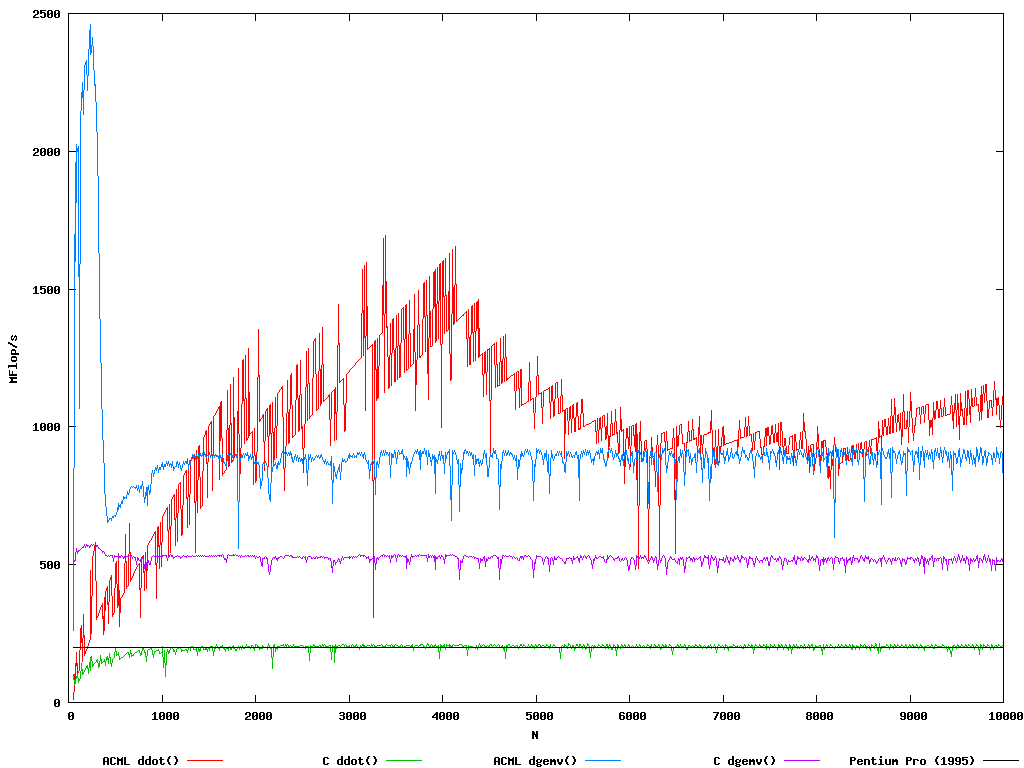
\includegraphics[height=3in]{blas12}
\end{center}
\note{
\begin{itemize}
 \item \texttt{pgcc -DACML -DBLAS1 -DBLAS2 -DBLAS3 blasSpeeds.c -lacml -pgf90libs -lpgftnrtl}
 \item \texttt{pgi/7.2 acml/4.1.0}
 \item opt2218  2.613 Ghz, 2flop/Hz,  5.226 Gflop
 \item Pentium Pro 200 Mhz (1995) 1 FPU 200MFlop/s Peak
\end{itemize}
 
 The Pentium Pro released in 1995 was available up to 200MHz. This CPU consisted of a single FPU (Floating Point Unit) that could execute up to 1 FP op per Hz.  This resulted in a max performance of 1flop*200MHz=200MFlop/s.  
 The point of this example was to show how even simple operations most result in performance at some small fraction of peak performance. Of the C code presented only the matrix*vector results in speed faster than the Pentium Pro's peak.
} % end note
\end{frame}

\begin{frame}{Blas 3}
\begin{center}
  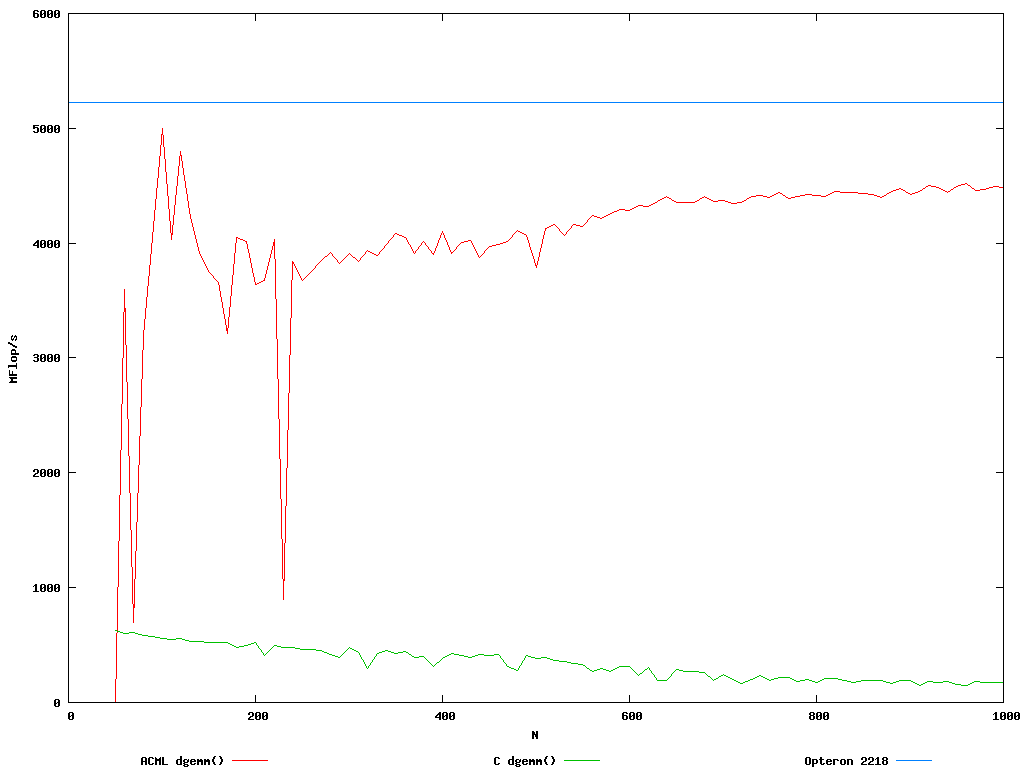
\includegraphics[height=3in]{blas3}
\end{center}
\note{
BLAS3 allows maximum performance to be extracted from the CPU without any fancy programming.  The C code because it really is a matrix vector product over N vectors results in the same poor performance as BLAS2.  This example compares results on a Opteron 2218 with a peak speed of 5226 Mflop/s and the achieved speed. \\
Opteron 2218 has 2 FPU's and operates at 2.613 Ghz. 
} %
\end{frame}

\section{Formating}
\subsection{Types}
\begin{frame}{Types}
 \begin{block}{Type Prefix}
  \begin{itemize}
   \item D Double
   \item S Single/Float
   \item C Complex
   \item Z Double Complex
    \item<2-> SGEMM() vs ZGEMM()
  \end{itemize}
 \end{block}
 \note{
 BLAS Supports 4 types.  Single, double, complex and double complex. A single letter D,S,C, or Z prefix a function for its use. For example DGEMM() is a matrix multiply when the matrixs are made of doubles, while SGEMM() is for floats/REAL's.  \\
Note that Single should be faster than double and double faster than complex and complex faster than double complex. \\
Last C has no native complex type. Most the BLAS libs define a struct with real and imag parts. Check the header of your BLAS lib for their own complex type. Fortran uses the native complex and complex*16 types.

 }%note
\end{frame}

\subsection{Naming}
\begin{frame}{Naming}
 \begin{block}{Naming}
  \begin{columns}[T]
   \begin{column}{5cm}
    \begin{itemize}
     \item GE - GEneral
     \item SY - Symmetric
     \item HE - HErmitian
     \item TR - TRiangular
     \item GB - General Band
    \end{itemize}
   \end{column}
   \begin{column}{5cm}
    \begin{itemize}
     \item SB - Sym. Band
     \item HB - Herm. Band
     \item SP - Sum. Packed
     \item HP - Herm. Packed
     \item TP - Triang. Packed
    \end{itemize}
   \end{column}
  \end{columns}
 \end{block}
\end{frame}

\begin{frame}{Transpose and CBlas}
 \begin{block}{Transpose and CBlas options}
  \begin{itemize}
   \item 'N' - No Transpose, CblasNoTrans
   \item 'T' - Transpose, CblasTrans
   \item 'C' - Conjugate Transpose, CblasConjTrans
   \item 'U' or 'L' CblasUpper, CblasLower Triangular
   \item 'N' or 'U' CblasNonUnit, CblasUnit Triangular
  \end{itemize}
 \end{block}
 \begin{block}{CBlas Memory Ordering}
  \begin{itemize}
   \item CblasRowMajor
   \item CblasColMajor
  \end{itemize}
 \end{block}
 See: \url{http://www.netlib.org/blas/blasqr.ps}
\end{frame}

\section{Code}
\subsection{Obtaining}
\begin{frame}{Obtaning the BLAS}
\begin{block}{Libraries}
 \begin{itemize}
  \item Intel:  MKL Math Kernel Library 
  \item AMD: ACML AMD Core Math Library
  \item Apple/PowerPC/Intel: VecLib
  \item IBM/Power: ESSL
  \item Intel/AMD/Alpha/IA64: GOTO Blas
  \item Any: ATLAS \url{http://math-atlas.sourceforge.net/}
 \end{itemize}
\end{block}
\note{
Each CPU manufacture publishes a library that implements the same functions. This allows code writen on one system to compile and link against the BLAS lib for another system and extract all the performance of the new cpu type.  Also manufactures release updated versions of their BLAS libraries to use new cpu features. Because of this every time you are on a new system ask your Admin what cpu type it uses and grab the newest version of the BLAS library for that cpu. \\
Most are free, and some will run on others, for example ACML will work on Intel Chips. A wonderful library that is free and works on most if not all CPU's is ATLAS.
} %note
\end{frame}

\subsection{Support Code}
\begin{frame}{Fortran vs. C}
  \begin{center}
  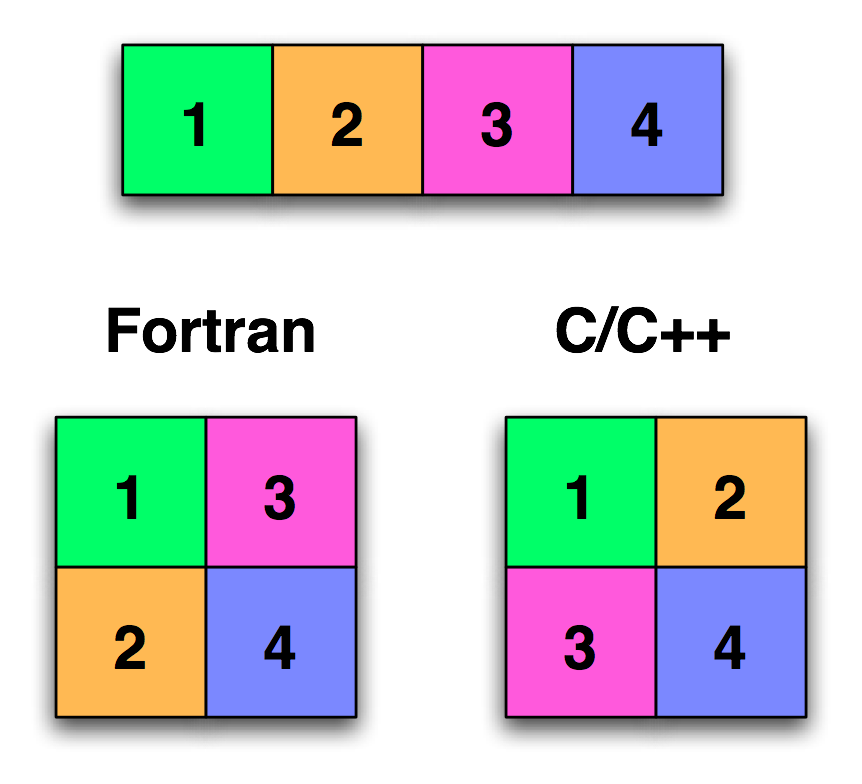
\includegraphics[height=3.0in]{matrixorder}  
  \end{center}
 \note{
 Fortran and C store matrixes in memory two differnt ways.  C/C++ store them in row major. That is the fastest varrying index is along the row of an array.  In fortran it is column major. Because of this BLAS libraries that are based on Fortran (most of them) even their C calls expect the matrix to be in column major order. \\

Note for C/C++ code matrixs can not be of the form M[i][j].  They must be of form M[i*j].  Fortran can use its normal form just fine M(j,i).
 } %note
\end{frame}
\begin{frame}{Fortran vs. C}
 \begin{block}{Fortran from C}
 \begin{itemize}
  \item BLAS1 or any array does not require special treatment.
  \item A transposed matrix in C is a non-transposed matrix in fortran:
  \begin{itemize}
   \item \texttt{dgemm('T', 'T', dim, dim, dim, 1, A, dim, B, dim, 0, C, dim);}
   \item \texttt{DGEMM('N', 'N', DIM, DIM, DIM, 1, A, DIM, B, DIM, 0, C, DIM)}
   \item When calling the fortran based BLAS from C
  \end{itemize}
 \end{itemize}
 \end{block}
\end{frame}
\end{document}
